\chapter{TTSP Design}

%-----------------------------------------------------------
% keywords: design goals and requirements, system architecture
%-----------------------------------------------------------
In the first part of this section, the design goals for TTSP and the requirements for the time synchronization in WSNs will be presented. Following these, the system architecture will be detailed. TTSP architecture will be presented in a bottom-up approach for every of its upper lying components.  

\setcounter{secnumdepth}{2}
\section{Design Goals and Requirements}
%-----------------------------------------------------------
% keywords: design goals
%-----------------------------------------------------------
\subsection{Design Goals}
The design goals declared here seek to address the problem introduced in chapter 1 and discussed in chapter 2.\\
The proposed system architecture, as later will be explained with detail, was implemented as a library on TinyOS \cite{conf/mdm/Levis06}. TinyOS is at the moment,  the most popular and extensively used operating system for sensor nodes. It started as a collaboration between the University of California, Berkeley in co-operation with Intel Research and Crossbow Technology, and has since grown to be an international consortium, the TinyOS Alliance. Being a open-source project, it has come to gather a strong community of contributors all around the world, with people from many scientific fields.\\
For the design goals, we'll start by looking at Figure \ref{designgoals}, where we can easily see the different layers between the hardware and software components that occur in a sensor node and those that shall happen with TTSP. TTSP shall interface directly with the application and the MAC protocol for the desired time precision it needs to its correct operation. The application and the MAC protocol will be able to declare its time precision requirements to TTSP, and TTSP shall give feedback to the application if those requirements are successfully achieved. TTSP shall also interact with the available operating system running on the node, in this case, the TinyOS core, in order to access the time counters incremented by the oscillator and make use of the radio. These cross-layer interactions will allow TTSP to assure a global and unique notion of time synchronization to all components in the nodes system.

\begin{figure}[!htb]
\begin{center}
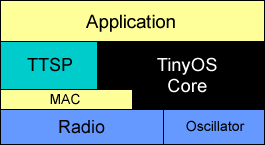
\includegraphics[scale=0.7]{./images/02-ttsp-hwsf_arch.png}
\end{center}
\caption{TTSP design goals.}
\label{designgoals}
\end{figure}

\subsection{Requirements}
%-----------------------------------------------------------
% keywords: requirements
%-----------------------------------------------------------
Here, follows a broad set of requirements that tries to address the time synchronization problem in WSNs. These requirements shall be fulfilled by a time synchronization protocol for WSNs. The requirements of a WSN protocol greatly differ from those found on a classic wired network, mainly due to its resources constraints. A WSN is often found with scarce resources at its disposal and it may be deployed on a hostile environment, where robustness to sensor node and communication link failures is also a key factor.

\subsubsection{Energy efficiency}
As with every other type of WSN protocol, a time synchronization protocol should take into account the limited energy resources that are available to the sensor nodes.

\subsubsection{Scalability}
A time synchronization protocol should not be limited to the  number of sensor nodes in the network. It should scale well with increasing number of sensor nodes.

\subsubsection{Precision}
A time synchronization protocol should fulfil the precision requirements of the applications. The need for precision or accuracy, may vary significantly depending on the specific application and the purpose of synchronization.

\subsubsection{Robustness}
Taking into account the energy constraints, the hostile environment that the WSN may be deployed and the volatile link quality of the communications in WSNs, it is expected that sensor nodes die, be removed from the network, or simply be unable to communicate between themselves for periods of time. The time synchronization protocol should remain valid and functional in the network, in case of failure of one or few of its sensor nodes. 

\subsubsection{Lifetime}
The time synchronization protocol in a WSN may provide time synchronization to its sensor nodes in a instantaneous fashion and act as long as the lifetime of the network.

\subsubsection{Scope}
A time synchronization may provide time synchronization to a local subset of the sensor nodes in the WSN, or a global time synchronization to all of the sensor nodes in the network.

\subsubsection{Cost and size}
The time synchronization protocol for WSNs should be developed with limited cost and size in mind. Adding dedicated hardware to every sensor node in the WSN for time synchronization may not be an option, as it can increase the cost for every sensor node and its overall size.

\section{Cross-layer interfaces}
%-----------------------------------------------------------
% keywords: cross-layer interfaces
%-----------------------------------------------------------
In order to fulfil its purpose, TTSP offers the application developer a specialized interface that, while still maintaining some similarities with conventional time synchronization protocol interfaces, has some special nuances that must be carefully taken into consideration. Mainly, the fact that, the cross-layer client of TTSP shall declare its tolerable threshold for time precision error, and/or its maximum synchronization period. The most relevant commands and events are illustrated in Figure \ref{crosslayer}.

\begin{figure}[!htb]
\begin{center}
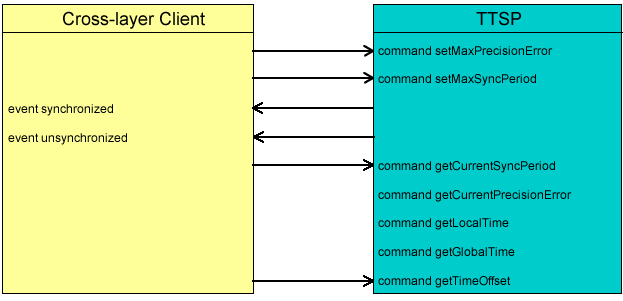
\includegraphics[scale=0.5]{./images/06-ttsp-crosslayer.png}
\end{center}
\caption{Cross-layer interfaces.}
\label{crosslayer}
\end{figure}

\section{System architecture}

%-----------------------------------------------------------
% keywords: system architecture
%-----------------------------------------------------------
As previously explained, TTSP allows its cross-layers applications to declare their time precision requirements, by stating their tolerable time precision error. These requirements are to be managed by an adaptive synchronization layer, which encapsulates all the adaptive logic, that is, contains the adaptive algorithm, maintains the state of the current precision error, synchronization period, reference clock node and requirements declared by its clients. This adaptive synchronization layer operates over two other classic synchronization layers: pair-wise synchronization and network-wide synchronization. Each one of these two layers encapsulates their own synchronization logic, that is, implement the algorithms for pair-wise and network-wide synchronization, and both are controlled by the adaptive synchronization layer. These two layers export a set of commands and events that allow the upper layer to take full control of the time synchronization techniques. This modular architecture for TTSP, allows one to easily substitute the pair-wise or network-wide synchronization algorithms and keep using the adaptive synchronization as long as they implement the set of commands and events that are used by the adaptive synchronization layer. Following a bottom-up approach, each one of these layers will be individually detailed below in Figure \ref{ttsparch}.

\begin{figure}[!htb]
\begin{center}
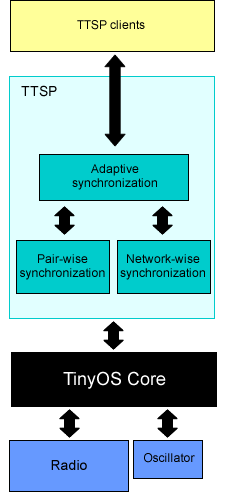
\includegraphics[scale=0.5]{./images/05-ttsp-design_goals.png}
\end{center}
\caption{TTSP architecture.}
\label{ttsparch}
\end{figure}

\subsection{Pair-wise synchronization}
%-----------------------------------------------------------
% keywords: pair-wise synchronization
%-----------------------------------------------------------
For pair-wise synchronization, TTSP uses a Sender-to-receiver message exchange scheme, mainly due to its low complexity and less complex requirements. This pair-wise synchronization will be refreshed periodically. By using a MAC-layer time-stamping with an approach like Sender-to-receiver, the high delay uncertainty found in this type of approach clearly decreases when compared with a Receiver-to-receiver. Making it a good choice instead of a Receiver-to-receiver with its inherent complexity.  By combining multiple estimates of the local time of a remote sensor node and using interpolation techniques it will be possible to compensate local clock skews.

\subsubsection{Synchronization through message exchange}
%-----------------------------------------------------------
% keywords: message exchange
%-----------------------------------------------------------
Assuming a Sender-to-receiver scheme, we're talking about synchronization between two or more nodes that are in the radio range of the sender and are able to exchange messages between themselves. Time synchronization between these nodes means that the nodes establish some relationship between their local clocks. The solution is for the sender to send a message containing a local time stamp to one of its neighbouring nodes, thus allowing the receiving node to synchronize with the senders clock. Although we've talked about only one receiving node, we can extend this message exchange to every receiving node that is in the radio broadcast area of the senders node.\\
Once a receiving node receives a synchronization message from the sender, he is now in possession of the senders local clock together with a local time stamp taken from of its own local clock of when the message was received. The receiving node is now able to calculate the offset between both clocks, and successfully adjust its logical clock to match with the senders local clock. This pair of  clock time stamps are commonly known as a synchronization point. Synchronization points are collected by the receiving nodes when a sender broadcasts its local clock.\\
In Figure \ref{syncmsg} it is possible to understand the synchronization process between two nodes through message exchange. Node i sends a message with a time-stamp of its local clock to node j. This process easily allows the receiving nodes to become aware of node i local clock.

\begin{figure}[!htb]
\begin{center}
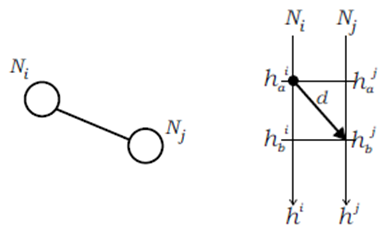
\includegraphics[scale=0.8]{./images/24-ttsp-sync_msg.png}
\end{center}
\caption{Two nodes synchronizing through message exchange.}
\label{syncmsg}
\end{figure}

But one problem persists with this technique, the receiving node cannot determine the exact delay of the message. It only knows for certain that the time-stamp of the local clock of the sender node was taken before he had received the message. Typically the uncertainty of the delay present in this message exchange can be decomposed in the following delays:

\begin{itemize}
\item the send time, lasting from when the application issues the send command to when the node actually starts trying to send; it is caused by kernel processing, context switches, and system calls, and hence varies with the current system load.
\item the (medium) access time, lasting from when the node is ready to send to when it actually starts the transmission; this is the time that is spent waiting for access to the wireless channel, and hence depends on the current network load.
\item the transmission time, which is the time taken to actually transmit the message, which depends only on the length of the message being transmited.
\item the propagation time, which is the time it takes for the radio signal to travel from the sender to the receiver; it is constant for any pair of nodes with constant distance, and is negligible compared to the other delay components in wireless sensor networks (since distances are small and radio signals travel very fast).
\item the receive time, lasting from the reception of the signal to the arrival of the data at the application.
\end{itemize}

Of all of these, only the transmission and the propagation time are deterministic. The send and receive time (and especially the uncertainty about them) and eventually the access time uncertainty can be reduced by implementing the time-stamping of outgoing and incoming messages at a very low level, for instance in the MAC layer.

\subsubsection{MAC-layer time-stamping}
%-----------------------------------------------------------
% keywords: MAC-layer time-stamping
%-----------------------------------------------------------
To minimize the delay uncertainty of the synchronization through message exchange, the use of time-stamping at the MAC-layer is essential, since it immediately limits three sources of delay uncertainties: access, transmit and receive times. In this case, the main message exchange delay comes from transmission and reception times at the radio chips. These delays can be further decomposed into 1) interrupt handling time, which is the delay between the radio chip raising and the micro-controller responding to an interrupt; 2) encoding time, which is the time it takes for the radio chip to encode and transform the message into a radio wave; 3) decoding time, which is the time for the radio chip at the receiver to transform the radio wave back into binary data; and 4) byte alignment time, which is the delay at the receiver to synchronize with the byte boundary at the physical layer. Thus, by using multiple time-stamps at the MAC-layer, when sending and receiving messages, it is possible to eliminate the jitter of interrupt handling and encoding/decoding times. 

\subsubsection{Synchronization rounds}
%-----------------------------------------------------------
% keywords: synchronization rounds
%-----------------------------------------------------------
Typically, two local clocks do not run at exactly the same speed. Therefore time synchronization has to be refreshed periodically, that is once these two clocks synchronize, they'll eventually start to drift apart from each other, mainly due to the sole characteristics of the hardware clock, the crystals oscillator might not have the same oscillating frequency, but also due to environmental conditions such as pressure and temperature which might affect the oscillating frequency of the crystal clocks. Thus, time synchronization in rounds becomes a continuous process, rounds follow each other seamlessly. So for every synchronization round a receiving node is able to collect one synchronization point. The duration of the round, or more commonly known as the synchronization period, depends on the available error budget and the amount of relative clock skew between the two clocks. As we will see below, one of the key factors in the adaptive synchronization will be adapting this synchronization period to satisfy the time precision error needed by the cross-layer applications.

\subsubsection{Skew compensation by combining multiple estimates}
%-----------------------------------------------------------
% keywords: skew compensation
%-----------------------------------------------------------
Although the synchronization may be done in rounds, through periodical broadcasted messages, one might take into consideration clock skew compensation techniques, which would minimize the offset from the two clocks in between synchronization points. As previously said, it's typical to find that different nodes have different clock skews, which is true, since the crystal used by the hardware clock might oscillate with a slight different frequency on each node, and thus, drift apart from each other at different rates.\\
In order to evaluate the clock skew between the nodes clocks, some tests were carried out on an already deployed test-bed, Tagus-SensorNet. The test involved six nodes and lasted for twenty-four hours. One node, the sink, was used as the clock reference for the remaining five nodes, these were initially synchronized at the beginning of the test and their clock skew was analysed during the following hours, that is, every node was allowed to collect only the initial synchronization point. The obtained results can be seen in Figure \ref{tsnclockskewchart}.\\

\begin{figure}[!htb]
\begin{center}
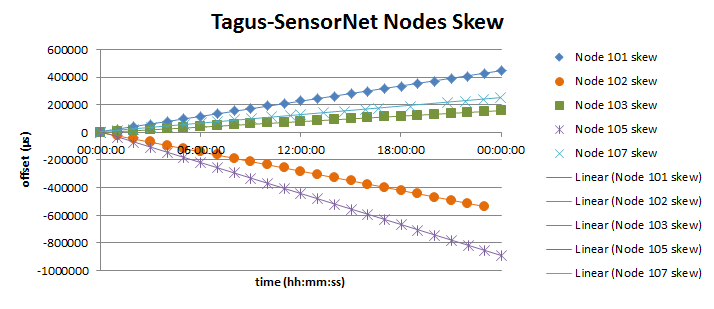
\includegraphics[scale=0.5]{./images/07-ttsp-tsn_skew.png}
\end{center}
\caption{Tagus-SensorNet nodes clock skew over 24 hours.}
\label{tsnclockskewchart}
\end{figure}

It's clear that once synchronized, each node starts to drift apart from the reference clock at a different rate. In order to get an approximated value of this rate, linear regression was used to find the best line that fits the collected dataset. The clock skews from each node were then obtained, and are shown in Table \ref{tsnclockskewtable}. 

\begin{table}[!htb]
\begin{center}
\begin{tabular}{|c|c|}
\hline
Node & Skew (ppm)\\ \hline
101 & 5,074 \\ \hline
102 &  -6,5 \\ \hline
103 &  1,797 \\ \hline
105 &  -10,376 \\ \hline
107 &  2,875 \\ \hline
\end{tabular}
\caption{Tagus-SensorNet nodes clock skew express in parts per milllion.}
\label{tsnclockskewtable}
\end{center}
\end{table}

Linear regression is the most widely used technique to predict the clock skew of a nodes clock, thus, allowing one to compensate for its clock skew with regard to its reference clock. As can be seen in Figure \ref{tsnclockskewerror}, the error obtained while predicting the above clock skews using linear regression assumes a bell-shaped distribution with its centre at 0 microseconds and a maximum error value of 57 microseconds.\\

\begin{figure}[!htb]
\begin{center}
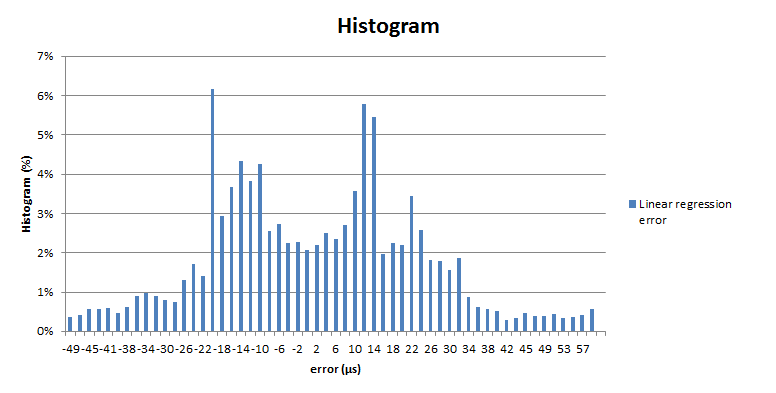
\includegraphics[scale=0.5]{./images/08-ttsp-tsn_histogram.png}
\end{center}
\caption{Error distribution while using linear regression to compute clock skews on Tagus-SensorNet.}
\label{tsnclockskewerror}
\end{figure}

This technique has a single parameter, that is the number of synchronization points that are accounted for when computing the clock skew. A large number of synchronization points can improve the regression quality, but requires a large amount of memory and might demand a considerable amount of processor occupation when done periodically. Linear regression implicitly allows one to compensate for the clock skew, but the clock skew is often variable during time, thus the postulated linear relationship between both clocks does not describe reality very well. In such situation, the number of samples accounted for should be small enough in order to minimize possible errors. Linear regression can be computed on-line, computed whenever a new sample is available. As we later experienced, with the adaptive mechanism being used, and synchronization periods being incremented and decremented between synchronization rounds, the best number of synchronization points found to adapt to the different rate at which samples would be collected, is between 4 and 8 samples.\\

\subsection{Network-wide synchronization}
%-----------------------------------------------------------
% keywords: network-wide synchronization
%-----------------------------------------------------------
For network-wide synchronization, the approach used for synchronization throughout the network is a master-slave scheme mainly also due to its low complexity and easy prediction of its behaviour while comparing to a peer-to-peer approach. The master will broadcast its local time to its neighbours, once these neighbours get synchronized with this master, they will then also start broadcasting to their neighbours.  In order to provide some redundancy to the master and easily adapt to network topology changes, a simple master election algorithm will ensure that a new root is elected once the previous one has cease to broadcast its local clock.

\subsubsection{Controlled flooding of broadcasted messages}
%-----------------------------------------------------------
% keywords: flooding
%-----------------------------------------------------------
The elected reference clock node, more commonly known as the root node, to which the whole network is being synchronized, keeps broadcasting its local clock within a certain period. Every other node that is within the broadcast radius of the root node can receive time-stamped messages from him, and collect synchronization points. When a node has collected enough synchronization points, he will be able to successfully compensate its clock skew with regard to the root node. By then, his in possession of the offset and the skew between both clocks. That node is considered synchronized with the root node and is now also able to start broadcasting its logical clock to its neighbouring nodes. The continuation of this process will eventually reassemble to a flooding of synchronization messages throughout the network. This flooding process takes advantage of the promiscuous communication medium that these wireless nodes use, allowing for a network-wide synchronization without a logic level hierarchy that many of the available time synchronization protocols for WSNs use.

\subsubsection{Master election mechanism}
%-----------------------------------------------------------
% keywords: master election mechanism
%-----------------------------------------------------------
One of the most critical problems found when using a master-slave approach for network-wide synchronization is that, the whole time synchronization process in the network, has one single-point of failure, that is the root node. It is important to introduce some redundancy in the network-wide synchronization process in case the root node for any technical reason fails or its broadcasted messages are subject to a permanent or temporary radio interference. The solution is to use a master election mechanism whenever the current root nodes is absent of the network. The root node is considered absent if for any reason the receiving nodes fail to collect a specific number of  synchronization points, which translates itself to a specific number of missed synchronization rounds. In order to prevent early master elections, the receiving nodes are configured to tolerate only a number of missing synchronization point, these optimal numbers as we later experienced, are from 3 to 4. These values are justified from a series of tests conducted in Tagus-SensorNet, in which lower values would trigger an early master election, which was caused by messages not being received by some of the receiving nodes, and a higher value would induce a slow detection of the master failure, thus a slower response and nodes would eventually be subject to variable time precision errors during that time.\\

Once the root node is declared absent from the network, the remaining nodes need to agree on a replacement for the root node. One here, could think of the hardware capabilities that could differentiate a node to be elected as replacement of the absent master, but since most WSNs test-beds, like Tagus-SensorNet lack some heterogeneity in hardware capabilities and platforms, that wouldn't make any differentiation. One solution would be to give priority to nodes that have plenty energy resources at their disposal, but that would almost always end with giving priority to nodes that are at the edges of the network and eventually create deep multi-hop chains between synchronizing nodes. The chosen solution for this priority, is the less complex and most predictable one. Nodes are elected as replacements for the root node by their logical identification. Every node gives high priority to a root node with a lower identification while synchronizing. That is, once the previous root node is declared absent from the network, each node declares itself as a possible candidate for being a replacement for the root node by starting broadcasting their local clock. Nodes will start a pair-wise synchronization with the self-elected root node that has the lower identification. Once they get synchronized with the new root node, they will also start broadcasting their logical clock. This broadcast contains the identification of the root node, so that in multi-hop scenarios, every node gets updated and synchronized with the new master.


\subsection{Adaptive synchronization}
%-----------------------------------------------------------
% keywords: adaptive synchronization
%-----------------------------------------------------------
By now, we've seen, that in order to maintain a long-term time synchronization among nodes, a periodic re-synchronization is needed, otherwise the timing of different nodes would drift apart as time passes. Thus, one needs to take into account that a less frequent re-synchronization requires a lower number of exchanged messages, thus, eventually lesser energy consumption by the sending and receiving nodes, but ultimately leads to a larger synchronization error, that is, time precision error. While a more frequent re-synchronization leads to a smaller time precision error but requires more energy. There is clearly a trade-off between energy expenditure and the achieved time precision error. The proposed adaptive synchronization layer shall find the minimum re-synchronization frequency (or equivalently maximum re-synchronization period) that can meet the desired  synchronization precision.\\
Therefore the adaptive synchronization layer is necessary to dynamically determine the re-synchronization period to be used in each round of synchronization based on the needed time precision error.

\subsubsection{Time precision error}
%-----------------------------------------------------------
% keywords: time precision error
%-----------------------------------------------------------
The adaptive synchronization must have knowledge of the required time precision error. As previously said, this precision error is declared by the cross-layer clients. Once the adaptive layer knows this value, it now needs to know how to systematically measure the current achieved time precision error. This measure is done at both the sender and the receiver. Each one should monitor this parameter in order to actuate over it.\\
The sender, more specifically the root node which is being used as the reference clock, has the responsibility of adjusting the synchronization period based on the precision error calculated from the broadcasts of the receiving nodes, once they get synchronized. One of the advantages of having a promiscuous physical medium and the fact that exchanged messages are broadcasted on it, is that the root node can listen to its synchronizing nodes broadcasts and measure the precision error of the synchronization messages they broadcast. In a multi-hop scenario these precision errors are obtained through relayed messages by the intermediary nodes. These intermediary nodes, which by then are already synchronized with the root node and aware of the time precision requirements are able to filter messages in case the calculated precision error is acceptable. Thus, in a multi-hop scenario the intermediary nodes have the responsibility of letting the root node know about unacceptable precision errors in the edges of the network.\\
On the other side, the receiver has a lesser significant responsibility but still important of managing the synchronization points already collected and employ filtering techniques on them, in order to assure an acceptable time precision error. This management is needed since, while adjusting to a new synchronization period, the already collected number of samples might induce some small precision error when calculating the logical clock time.

\subsubsection{Synchronization period}
%-----------------------------------------------------------
% keywords: synchronization period
%-----------------------------------------------------------
As previously said, only the root node has the responsibility of adjusting the synchronization period. The initial synchronization period is statically pre-configured on all nodes, and should reflect a period that is known to be safe to start with. The following synchronization periods to be used by the root node are adjusted by the adaptive algorithm, which reflect the current time precision error. This adaptive adjustment is made on the sole basis of the current time precision error. The adjustment is made using a \ac{MIMD} strategy. The concept is straightforward, if the current time precision error is larger than  the requested time precision, it means that the synchronization period is too high, therefore the synchronization period should decrease by a certain factor. On the other hand, if the time precision error is smaller than the requested time precision error, that translates into a lower synchronization period, and thus, it could be increased by a certain factor. This procedure is seen as a transition state, in which there is no knowledge about the best synchronization period to be used, which are mainly influenced by the network topology (multi-hop distances), node crystals and the environment itself. After the adaptive algorithm stabilizes, that is, after it found at which period it achieves an acceptable time precision error on all nodes, it then stops adjusting the synchronization period. This adaptive algorithm can be best described by a finite-state machine, depicted in Figure \ref{statemac}  which is composed by three distinct states. 

\begin{figure}[!htb]
\begin{center}
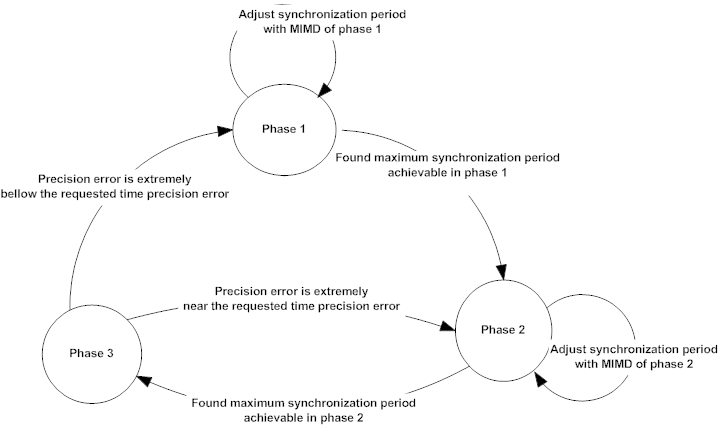
\includegraphics[scale=0.5]{./images/25-ttsp-machine_state.png}
\end{center}
\caption{Finit-state machine for the synchronization period adjustment algorithm.}
\label{statemac}
\end{figure}

The finite-state machine used in the adaptive algorithm has three distinct phases. In each phase of this finite-state machine the synchronization period is adjusted. Although, each phase is characterized by having its particular \ac{MIMD} granularity level, starting with a lower \ac{MIMD} granularity level in phase 1 while finishing with a higher \ac{MIMD} granularity level at phase 3. The transition conditions on the first two phases are the same, with the sole objective to quickly assess the maximum synchronization period that is possible to achieve under the given conditions, that is, to find the maximum synchronization period that is possible to be achieved with that \ac{MIMD} granularity level while maintaining an acceptable precision error. For the first and second phase, once this maximum synchronization period is obtained, there is a transition to a phase with a higher \ac{MIMD} granularity level. On the third and last phase, the \ac{MIMD} granularity level is sufficient high that only minimal changes to the synchronization period are taken place, this can be seen as entering a stabilization process in the adjustment of the synchronization period. The transition conditions in this phase differ from the previous two, since the objective here is to guarantee that significant precision error changes with the achievable time synchronization period are mitigated by finding a new best suitable time synchronization period.

In order to support the better explanation of this finite-state machine and the underlying decisions taken by the synchronization period adjustment algorithm, a flowchart of every decision and action taken by this algorithm can be seen Figure \ref{flow} followed by a detailed explanation of each phase.

\begin{figure}[!htb]
\begin{center}
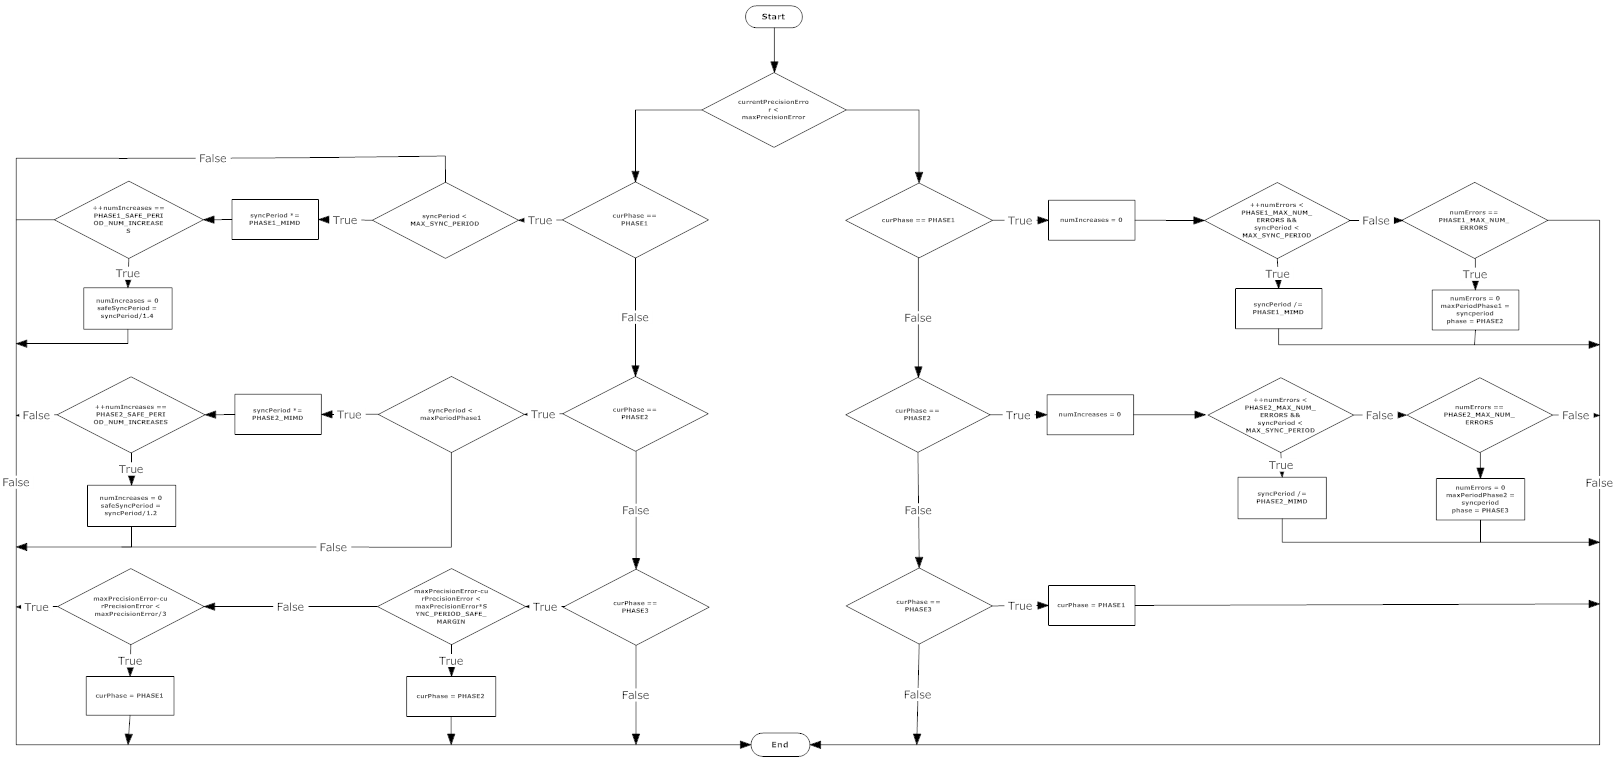
\includegraphics[scale=0.4,angle=90]{./images/26-ttsp-flowchart.png}
\end{center}
\caption{Detailed flowchart of the synchronization period adjustment algorithm.}
\label{flow}
\end{figure}

\clearpage

The first and initial phase, known to be as phase 1, is triggered on the root node after the first synchronization message from one of its receiving nodes is received, that is, once one neighbouring node gets synchronized and starts to broadcast its logical clock time. From that on, and on every synchronization message received in a synchronization round from its synchronized neighbours, the root adjusts the synchronization period to meet the required time precision error. The root node filters synchronization messages by its synchronization round identification, so that it only adjusts the synchronization period once in a synchronization round. Although, there are cases in which one node has an acceptable error, but another don't, in this case, the root needs to filter messages by synchronization rounds but also take into consideration the time precision error of the node, eventually giving priority to adjustments that keep the overall time precision error lower. For every two consecutive period increases, the algorithm records a safe period, which it will use as a fall-back when it receives a non-consecutive number of synchronization messages with an unacceptable precision error and needs to drastically decrease the synchronization period. The MIMD granularity used in this phase is typically higher than the other remaining phases, since there is no knowledge at that moment from the conditions of the network. The transition from this phase is done after a certain number of non-consecutive synchronization messages with a time precision higher than the accepted. When transitioning from this phase, the adaptive algorithm has the knowledge of the maximum synchronization period that it can sustain for the given network conditions. As said, this transition will be made after the maximum synchronization period is known, this will typically involve achieving a higher time precision error, which will result in a decrease in the time synchronization period to a known safe period, as previously explained. The next phase, will take this knowledge into consideration.

The second phase of the adaptive algorithm, known as phase 2, is somehow similar with the first phase, it also can be described as a discovery phase, but now with the difference that we know the maximum synchronization period that can be achievable under an acceptable precision error, thus the MIMD granularity used in this phase is smaller than the used on the previous phase, since we're are interested in maximizing the synchronization period closer to the previous known maximum synchronization period but without the precision errors. Like in the previous phase, the algorithm quickly reacts to small variations of the achieved time precision error in order to keep it under the required precision. This phase is also considered a transition state, that is, the synchronization period can still fluctuate significantly between the two distinct thresholds that it knows, the safe synchronization period and the maximum synchronization period obtained from the previous phase. The transition from this phase is done after a certain number of consecutive increases and a decrease or a certain number of decreases and an increase.

The third and last phase of the adaptive algorithm, phase 3, can be considered as a stabilization phase, since once in this phase the current synchronization period is considered safe and lower the maximum synchronization period where the unacceptable time precision errors were detected. In this phase, the MIMD granularity is very small since for most cases the precision error should be within the required thresholds and not be subject to high variations. This phase can be grossly characterized by a steady synchronization period. Nonetheless, if by any means, the time precision error keeps getting close to the threshold of the requested time precision error for a long period of time, that is, a certain number of synchronization round, a transition to phase two will be made, since it is considered that the current synchronization period is not suitable any more. The same procedure is made for when the time precision error is well below the requested time precision error and close to zero, but instead, a transition will be made to phase one, because of its higher MIMD granularity.

\subsubsection{Fast synchronization}
%-----------------------------------------------------------
% keywords: fast synchronization
%-----------------------------------------------------------
One needs to take into consideration that when adaptively adjusting the synchronization period in a network of sensor nodes, new nodes might be added to the network and it might be requested that they should get as quickly as they can synchronized with the rest of the network nodes. This is somehow inefficient while on a large synchronization period, since typically a node needs to collect a certain number of synchronization points before it gets synchronized with remain nodes. Thus, on those cases the new node would have to wait for N times the large synchronization period, where N is the number of necessary synchronization points, which would consume a considerable amount of time and  has proven not to be acceptable in networks which might have nodes being turned off for maintenance and added back again with some high frequency. For those cases a fast synchronization mechanism was introduced to quickly detect and synchronize new nodes in the network. The concept is that a node will discard synchronization messages that contain a large synchronization period, thus eventually declaring itself the root node since all synchronization messages from possible root nodes have been discarded. Once it declared itself the root node, it will start to broadcast with its identification which will be received by neighbouring nodes which are already synchronized with the correct root node. Upon receiving a synchronization message from a root that is not his root and not in conditions to be a root, the receiving node will trigger a fast synchronization mechanism which will broadcast a consecutive number of synchronization messages within a short period of duration. The new node will then be aware of the real root node and also be able collect the necessary synchronization points in order to synchronize with him. The consecutive number of messages are sent using the initial synchronization period, which is quite small compared to the possible synchronization period that might be in use, thus, this procedure only takes up to N times the initial synchronization period, which by convention is much smaller than the larger synchronization period.\\

To briefly summarize TTSP architecture, it can be best seen as a set of common techniques that are used by many of the existent time synchronization protocols, but with the exception, that here, they are embedded in an adaptive mechanism in order to meet specific requirements that are demand by TTSP clients. Thus, these tools are to be used with regard to the desired time precision. They are used by the adaptive mechanism in order to cope with the effort necessary to achieve the desired time precision. Although many of these techniques are broadly used by other time synchronization protocols, most of them required a significant number of modifications or complements in order to be usable in a adaptive fashion, for example, the compensation skew technique, which requires a specific number of samples and a better management and filtering of these samples while adjusting the synchronization period.\\
